\chapter{Stability, Feedback Control \& Luenberger Observer for Balancing an Inverted Rotary Pendulum}

The purpose of this lab is to study the rotary pendulum system and to develop a control technique that balances the pendulum around an equilibrium using partial state feedback and a linear observer. In the lab, you will first use full state feedback and pole placement techniques to develop a controller that balances the inverted pendulum. Then, you will carry out the same task for the case where you do not have access to the full state information. To do this, you will develop a Luenberger observer to estimate the states that you do not have access to and you will use the estimated states to develop a controller that balances the inverted pendulum.
\begin{figure}[htb!]
    \centering
    \includegraphics[width=.3\linewidth]{eps/lab_3/quanser.eps}
    \caption{Qanser SRV02 with pendulum module, shown in an inverted orientation~\cite{Q-Flex-Beam}.}
    \label{fig:lab3_plant}
\end{figure}

\section{Key Concepts}
\subsection{Modelling the Beam Using the Euler-Lagrange Equation}
From previous mechanics courses, you should be familiar with modelling physical systems using first principles (i.e., Newton's Laws). For simple systems, this first principles approach to modelling a physical system is relatively straightforward and works very well; however, for more complicated systems, things can get ugly very quickly. For modelling our rotary flexible beam, it is easier to use a more modern approach to modelling that employs the \emph{Euler-Lagrange equation}.

The Euler-Lagrange equation is a second-order partial differential equation that will help you find the equations of motion for our physical system. Before presenting the Euler-Lagrange equation, we must first introduce some mathematical objects and notation that have strong physical interpretations.

To describe the configuration of the physical system relative to some reference configuration, we use coordinates (not to be confused with the coordinate axes shown in Figure~\ref{fig:lab1_rotary_flexible_beam} - we're talking about variables $\theta$ and $\alpha$ here) which we call the \emph{generalized coordinates} of the system, and we denote the $i^{th}$ generalized coordinate by $q_i$. We define the kinetic and potential energies of the system by functions of the generalized coordinates and their time derivatives, and denote them by $T$ and $V$, respectively. To summarize the dynamics of our physical system, we use the function $L$ (called the \emph{Lagrangian} of the dynamical system) which is defined by
\[
    L=T-V.
\]
In modelling a physical system, we must also consider external forces applied to the system. We do this by defining a \emph{generalized force} for each generalized coordinate $q_i$ which takes into account the effects of externally applied forces (or torques if $q_i$ is an angle) that are excluded from $V$ (e.g., the force of gravity is a potential force, not a generalized force). We denote the generalized force for $q_i$ by $Q_{q_i}$.
The Euler-Lagrange equation is then given as follows:
\begin{equation}\label{equation:lab1_lagrange_equns}
    \frac{d}{dt} \Bigg(\frac{\partial L}{\partial \dot{q_i}}\Bigg)  - \frac{\partial L}{\partial q_i} = Q_{q_i}.
\end{equation}
To find the equation of motion for a particular coordinate $q_i$, all one must do is find $L$, $V$ and then evaluate~\eqref{equation:lab1_lagrange_equns}. For the rotary pendulum system, our coordinates will be the rotary shaft angle, $\theta$, and the pendulum rod angle, $\alpha$, so that our coordinate vector is $q(t)^T=[\theta(t) \; \alpha(t)]$. See Figure~\ref{fig:lab2_rotary_pendulum} for what these coordinates look like in the physical system.

\begin{figure}[H]
    \centering
    \begin{subfigure}{.4\textwidth}
        \centering
        \includegraphics[width=\textwidth]{eps/lab_2/quanser.eps}
        \caption{}
    \end{subfigure}\hfill
    \begin{subfigure}{.4\textwidth}
        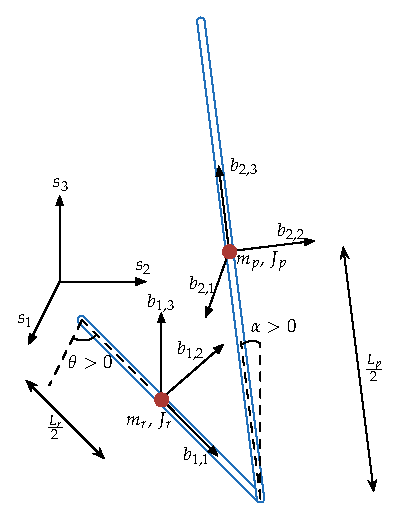
\includegraphics[width=\textwidth]{eps/lab_2/rotary_pendulum_edit.eps}
        \caption{}
    \end{subfigure}
    \caption{(a) Physical rotary pendulum system~\cite{Q-Flex-Beam}; (b) model of the physical system with two rigid bodies connected together, where rigid body 1 (rotary shaft) rotates in the horizontal plane and rigid body 2 (pendulum rod) rotates in the vertical plane. The reference coordinate axes are shown by $\{s_1,s_2,s_3\}$, and the body coordinate axes for rigid bodies 1 and 2 are shown by $\{b_{1,1},b_{1,2}, b_{1,3}\}$ and $\{b_{2,1},b_{2,2},b_{2,3}\}$, respectively. The centres of mass for bodies 1 and 2 are shown in red; the horizontal rotation angle, $\theta$, the vertical rotation angle, $\alpha$, are shown. Important distances are labelled.}
    \label{fig:lab2_rotary_pendulum}
\end{figure}

We will consider two cases: one when the pendulum is in its \textbf{downwards} position (i.e.\ \( \alpha=\pi \)), and one in its \textbf{inverted} position (i.e.\ \( \alpha=0 \)).

\subsection{Setting up the Rotary Pendulum}\label{subsection:lab2_setup}
First, let us assemble and wire the physical system. Examine the close-up assembly shown in Figure~\ref{fig:lab1a_assembly}, and replicate this at your workstation. Note that the high-gear configuration is used here. Use the wiring diagram shown in Figure~\ref{fig:lab1a_wiring} to connect the rotary pendulum to a power source and the data acquisition board.
\begin{figure}[htb!]
    \centering
    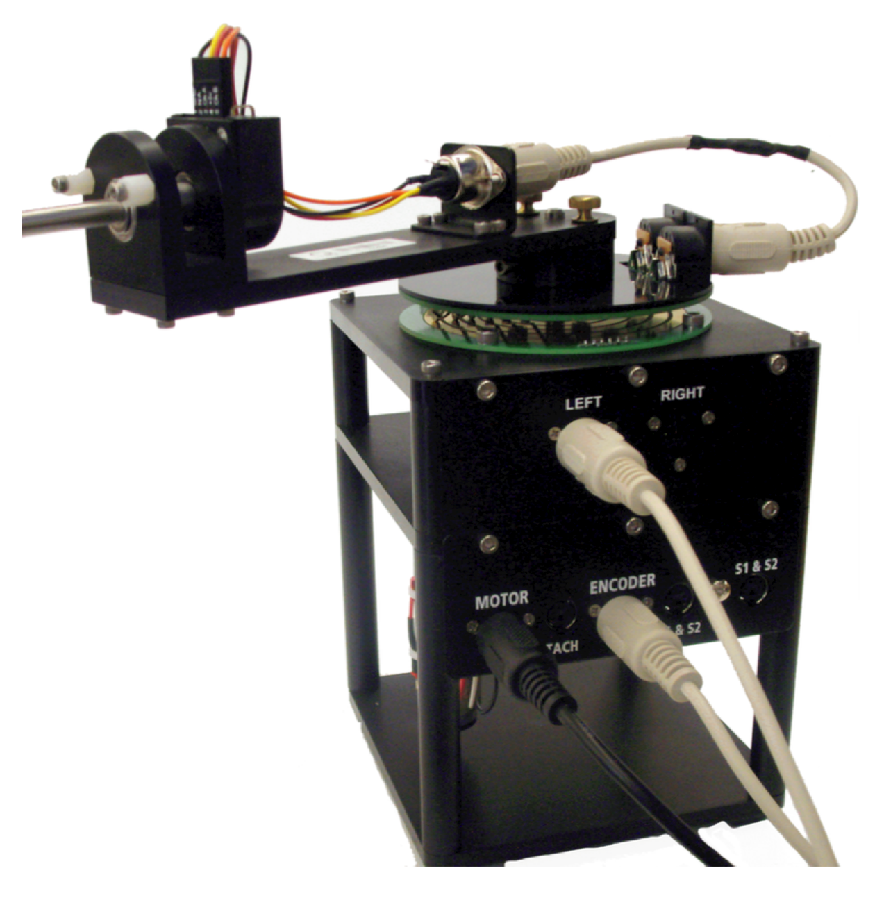
\includegraphics[width=.3\linewidth]{eps/lab_2/assembly.eps}
    \caption{A close-up of the assembly of the rotary pendulum module and the Quanser SRV02 plant~\cite{Q-Flex-Beam}.}
    \label{fig:lab1a_assembly}
\end{figure}
\begin{figure}[htb!]
    \centering
    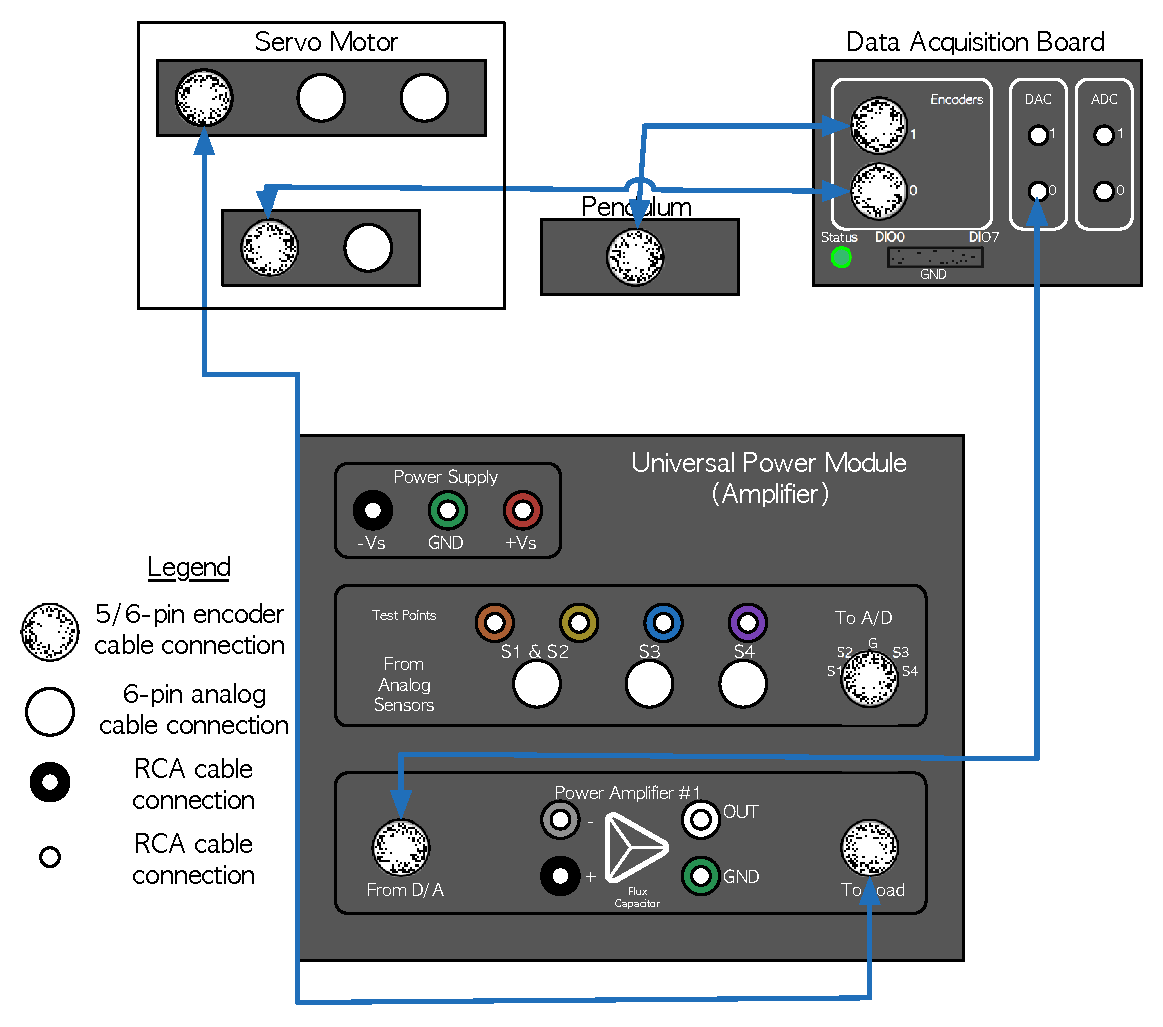
\includegraphics[width=.7\linewidth]{eps/lab_2/wiring.eps}
    \caption{A wiring diagram for the Quanser SRV02 and rotary pendulum module.}
    \label{fig:lab1a_wiring}
\end{figure}

\textbf{Note:} The power amplifier must be turned on before you can experiment with the physical system. The power switch is located at the back of the amplifier (good luck finding it). Make sure to turn off the power amplifier before you leave the lab.

\subsection{Feedback Gain and Pole Placement}\label{subsection:feedback}
Recall that for $A \in \mathcal{M}^{n \times n}(\mathbb{R})$ and for $B \in \mathbb{R}^n$, if the pair $(A,B)$ is controllable, then there exists a transformation $T \in \mathcal{M}^{n \times n}(\mathbb{R})$ where $\text{det}(T) \not = 0$ and
\begin{equation}\label{eq:A_tilde}
    \tilde{A} = TAT^{-1} =
    \left[\begin{array}{c c c c c}
            0      & 1      & 0    & \dots  & 0        \\
            0      & 0      & 1    &        & 0        \\
            \vdots & \vdots &      & \ddots & \vdots   \\
            0      & 0      & 0    & 0      & 1        \\
            -a_0   & -a_1   & -a_2 & \dots  & -a_{n-1}
        \end{array}\right]
\end{equation}
where $\chi_{A} = \chi_{\tilde{A}} = s^n + a_{n-1} s^{n-1} + \dots + a_1 + a_0$ (i.e., $\tilde{A}$ is uniquely determined by the coefficients of the characteristic polynomial of $A$), and
\[
    \tilde{B} = TB =
    \left[\begin{array}{c}
            0      \\
            0      \\
            \vdots \\
            1
        \end{array}\right],
\]
which is called the canonical controllable form (recall that $(A,B)$ is controllable if and only if $(\tilde{A},\tilde{B})$ is controllable since system controllability is invariant under similarity transformations). To find an appropriate feedback gain $K$ for your system~\eqref{equation:lab3_feedback} that will place the system's poles in $\mathbb{C}^-$, you will first design a feedback gain $\tilde{K}$ for the transformed system and then transform $\tilde{K}$ into $K$. To do that, design $\tilde{K} = [k_0, \; k_1, \; \dots, \; k_{n-1}]$ so that you obtain the desired poles:
\[
    \tilde{A}-\tilde{B}\tilde{K} =
    \left[\begin{array}{c c c c  c}
            0          & 1          & 0          & \dots  & 0                  \\
            0          & 0          & 1          &        & 0                  \\
            \vdots     & \vdots     &            & \ddots & \vdots             \\
            0          & 0          & 0          & 0      & 1                  \\
            -(a_0+k_0) & -(a_1+k_1) & -(a_2+k_2) & \dots  & -(a_{n-1}+k_{n-1})
        \end{array}\right]
\]
which yields $\chi_{(\tilde{A}+\tilde{B}\tilde{K})} = s^n + (a_{n-1}+k_{n-1})s^{n-1} + \dots + (a_1 + k_1) + (a_0 + k_0)$. In class, you found an explicit formula for computing the transformation $T$:
\[
    T=\mathcal{C}_{(\tilde{A},\tilde{B})} \mathcal{C}_{(A,B)}^{-1}.
\]

\subsection{Luenberger Observers}
Let us denote the state estimate by $\hat{\mathbf{x}}(t)$. David G. Luenberger proposed the following linear state observer~\cite{david1971introduction}:
\begin{equation}\label{lab3_equ:luenberger}
    \mathbf{\dot{\tilde{x}}}(t)=A\hat{\mathbf{x}}(t)+Bu(t)+L(\mathbf{y}(t)-C\hat{\mathbf{x}}(t)),
\end{equation}
where $L$ is the observer gain. Note that the input and measured output data are both used in~\eqref{lab3_equ:luenberger}. The observer in~\eqref{lab3_equ:luenberger} is composed of two parts: the first part, $A\hat{\mathbf{x}}(t)+Bu(t)$, is the rate of change of $\hat{\mathbf{x}}(t)$ as computed by the physical system's state-space model; the second part, $L(\mathbf{y}(t)-C\hat{\mathbf{x}}(t))$, is the difference between the observed output and the estimated output, scaled by the observer gain. Notice that without the second term, ~\eqref{lab3_equ:luenberger} becomes familiar:
\begin{equation}\label{lab3_equ:luenberger_simple}
    \mathbf{\dot{\hat{x}}}(t)=A\hat{\mathbf{x}}(t)+Bu(t).
\end{equation}
Let us denote the estimation error by $\tilde{\mathbf{x}}(t)$ and define it by $\tilde{\mathbf{x}}(t) = \mathbf{x}(t)-\hat{\mathbf{x}}(t)$. If one were to study the estimation error of the simplified observer~\eqref{lab3_equ:luenberger_simple}, then they would conclude that $\tilde{\mathbf{x}}(t)$ would go to zero when $\text{spec}(A) \subset \mathbb{C}^-$, as the error dynamic for~\eqref{lab3_equ:luenberger_simple} is
\begin{align*}
    \mathbf{\dot{\tilde{x}}}(t) & = A \left(\mathbf{x}(t)-\hat{\mathbf{x}}(t)\right)+Bu(t) - Bu(t) \\
                                & = A\tilde{\mathbf{x}}(t).
\end{align*}
That is, when matrix $A$ has all of its eigenvalues in the left half-plane, then the state estimate would converge to the actual state. But this convergence depends on the physical system's dynamics (thus the convergence rate can be quite slow, depending on the system) and the spectral constraints on $A$ are very restrictive. In contrast, the error dynamic for the Luenberger observer in~\eqref{lab3_equ:luenberger} is
\begin{equation}\label{lab3_equ:luenberger_error}
    \mathbf{\dot{\tilde{x}}}(t) = (A-LC) \tilde{\mathbf{x}}(t).
\end{equation}
Thus one can design an observer gain $L$ such that $\text{spec}(A-LC) \subset \mathbb{C}^-$ (i.e., an \emph{asymptotically stable observer}) and one can tune $L$ such that $\hat{\mathbf{x}}(t)$ converges to $\mathbf{x}(t)$ fast enough for the desired application. An important question to ask is, ``when does such an observer exist"? In class, you proved that one can build an observer with these properties when $(C,A)$ is \emph{detectable}.


\section{Background Information}\label{section:lab3_prelab}
The following sections will provide relevant matrices/equations for the lab. Don't get too caught up in the calculations, just understand the rough ideas, and use the provided matrices/equations as required.

\subsection{Equations of Motion}
We first wish to write down the EOMs for the rotary pendulum system (for coordinates \( \theta \) and \( \alpha \)) using~\eqref{equation:lab1_lagrange_equns}. Since the rotary shaft is actuated and the pendulum rod is not, and accounting for viscous friction, one can infer that $Q_\theta = \tau - B_r \dot{\theta} $ and $Q_\alpha = -B_p \dot{\alpha}$, where $\tau$ is the torque applied by the servo motor, and $B_r$, $B_p$ are the viscous damping coefficients for the rotary shaft and pendulum rod, respectively. Deriving $T$ and $V$ for the Lagrangian is not in the scope of this course, so they are provided below:
\begin{equation*}
    \begin{cases}
        T = \left(\frac{1}{2} m_p L_{r}^2 + \frac{1}{8} m_p L_{p}^2 - \frac{1}{8} m_p L_{p}^2 \cos^2(\alpha) + \frac{1}{2} J_r\right) \dot{\theta}^2 + \left(\frac{1}{2} J_p + \frac{1}{8} m_p L_{p}^2 \right) \dot{\alpha}^2 - \frac{1}{2} m_p L_p L_r \cos(\alpha) \dot{\theta} \dot{\alpha} \\
        V = \frac{1}{2} m_p L_p g \cos(\alpha)
    \end{cases}
\end{equation*}
where $J_p$, $m_p$, and $L_p$ are the moment of inertia about the centre of mass, mass, and length of the pendulum, respectively; $J_r$, $m_r$, and $L_r$ are the moment of inertia about the centre of mass, mass, and length of the rotary shaft, respectively; and $g$ is the acceleration due to gravity (on earth).
We compute the following sets of equations:
\[
    \begin{cases}
        \frac{\partial{L}}{\partial \theta}=0                                                                                                                                                      \\
        \frac{\partial L}{\partial \dot{\theta}}=\left( m_pL_r^2 +\frac{1}{4} m_p L_p^2-\frac{1}{4}m_pL_p^2\cos^2(\alpha)+J_r\right)\dot{\theta} - \frac{1}{2} m_pL_pL_r\cos{(\alpha)}\dot{\alpha} \\
        \frac{d}{dt} \left(\frac{\partial L}{\partial \dot{\theta}}\right)= \left(m_pL_r^2 +\frac{1}{4}m_pL_p^2-\frac{1}
        {4}m_pL_p^2\cos^2(\alpha)+J_r\right)\ddot{\theta} + \frac{1}{2}m_pL_p^2\sin{(\alpha)}\cos{(\alpha)} \dot{\alpha}\dot{\theta}                                                               \\+ \frac{1}{2}m_pL_pL_r\sin{(\alpha)}\dot{\alpha}^2-\frac{1}{2}m_pL_pL_r\cos{(\alpha)}\ddot{\alpha} \\
    \end{cases}
\]
\[
    \begin{cases}
        \frac{\partial L}{\partial \alpha}=\frac{1}{4}m_pL_p^2\cos{(\alpha)}\sin{(\alpha)}\dot{\theta}^2+\frac{1}{2}m_pL_pL_r\sin{(\alpha)}\dot{\theta}\dot{\alpha}+ \frac{1}{2}m_pL_pg\sin{\alpha} \\
        \frac{\partial L}{\partial \dot{\alpha}}= \left(J_p+\frac{1}{4}m_pL_p^2\right)\dot{\alpha}-\frac{1}{2}m_pL_pL_r\cos{(\alpha)}\dot{\theta}                                                   \\
        \frac{d}{dt} \left(\frac{\partial L}{\partial \dot{\alpha}}\right)= \left(J_p+\frac{1}{4}m_pL_p^2\right)\ddot{\alpha}+\frac{1}{2}m_pL_pL_r\sin{(\alpha)}\dot{\theta}\dot{\alpha}-\frac{1}{2}m_pL_pL_r\cos{(\alpha)} \ddot{\theta}
    \end{cases}
\]
Thus, via the Euler-Lagrange equation we get the following EOMs for the coordinates. For \( \theta \):
\begin{align*}
     & \left(m_p L_{r}^{2} + \frac{1}{4} m_p L_{p}^{2} - \frac{1}{4} m_p L_{p}^{2} \cos^2(\alpha) + J_r\right) \ddot{\theta} - \frac{1}{2} m_p L_p L_r \cos(\alpha) \ddot{\alpha} \\
     & + \frac{1}{2} m_p L_{p}^{2} \sin(\alpha)\cos(\alpha) \dot{\theta}\dot{\alpha} + \frac{1}{2}m_p L_p L_r \sin(\alpha) \dot{\alpha}^{2} = \tau - B_r \dot{\theta}
\end{align*}
And for \( \alpha \):

\begin{align*}
     & -\frac{1}{2} m_p L_p L_r \cos(\alpha) \ddot{\theta} + \left(J_p + \frac{1}{4} m_p L_{p}^{2}\right)\ddot{\alpha} - \frac{1}{4} m_p L_{p}^{2} \sin(\alpha)\cos(\alpha) \dot{\theta}^{2} \\
     & - \frac{1}{2} m_p L_{p} g \sin(\alpha) = - B_p \dot{\alpha}
\end{align*}

\subsection{Linearization}
Note that these EOMs are nonlinear, so we wish to linearize these equations about an equilibrium point. Recall that to linearize a multivariate function \( f \) of variables \( z^T = [\theta \; \alpha \; \dot{\theta} \; \dot{\alpha} \; \ddot{\theta} \; \ddot{\alpha}] \) around an equilibrium point \( z_{0}^T = [\theta_0 \; \alpha_0 \; \dot{\theta}_0 \; \dot{\alpha}_0 \; \ddot{\theta}_0 \; \ddot{\alpha}_0] \), we use
\[
    f_\text{lin} = f(z_0) + \left(\frac{\partial f(z)}{\partial \theta}\right) \bigg|_{z_0}  (\theta - \theta_0) +  \left(\frac{\partial f(z)}{\partial \alpha}\right) \bigg|_{z_0}  (\alpha - \alpha_0) + \dots +  \left(\frac{\partial f(z)}{\partial \ddot{\alpha}}\right) \bigg|_{z_0}  (\ddot{\alpha} - \ddot{\alpha}_0)
\]
We consider two cases for the equilibrium point.

\subsubsection*{Downwards Position (\( \theta_0=0, \alpha_0=\pi \))}
For the generalized coordinate \( \theta \), we compute
\[
    \left(m_p L_{r}^{2} + J_r\right) \ddot{\theta} + \frac{1}{2} m_p L_p L_r \ddot{\alpha} = \tau - B_r \dot{\theta}
\]
And for the generalized coordinate \( \alpha \), we compute
\[
    \frac{1}{2} m_p L_p L_r \ddot{\theta} + \left(J_p + \frac{1}{4} m_p L_{p}^{2}\right)\ddot{\alpha} + \frac{1}{2} m_p L_{p} g \alpha = - B_p \dot{\alpha}
\]

\subsubsection*{Inverted Position (\( \theta_0=0, \alpha_0=0 \))}
For the generalized coordinate \( \theta \), we compute
\[
    \left(m_p L_{r}^{2} + J_r\right) \ddot{\theta} - \frac{1}{2} m_p L_p L_r \ddot{\alpha} = \tau - B_r \dot{\theta}
\]
And for the generalized coordinate \( \alpha \), we compute
\[
    -\frac{1}{2} m_p L_p L_r \ddot{\theta} + \left(J_p + \frac{1}{4} m_p L_{p}^{2}\right)\ddot{\alpha} - \frac{1}{2} m_p L_{p} g \alpha = - B_p \dot{\alpha}
\]

\subsection{State-Space Representation}
In order to find the state space representation, we first write the linearized EOMs in matrix form, i.e.,
\[
    \left[\begin{array}{c c}
            e_{11} & e_{12} \\
            e_{21} & e_{22}
        \end{array}\right]
    \left[\begin{array}{c}
            \ddot{q}_{1} \\
            \ddot{q}_{2}
        \end{array}\right] +
    \left[\begin{array}{c c}
            f_{11} & f_{12} \\
            f_{21} & f_{22}
        \end{array}\right]
    \left[\begin{array}{c}
            \dot{q}_{1} \\
            \dot{q}_{2}
        \end{array}\right] +
    \left[\begin{array}{c}
            g_1 \\
            g_2
        \end{array}\right] =
    \left[\begin{array}{c}
            \tau_1 \\
            \tau_2
        \end{array}\right],
\]
and group all non double-derivative terms to the right. We can now explicitly solve for $\left[\begin{array}{c}
            \ddot{\theta} \\
            \ddot{\alpha}
        \end{array}\right]$ and put it in a relatively compact form. Letting our state be
\[
    \mathbf{x}(t) =
    \left[\begin{array}{c}
            \theta(t)       \\
            \alpha(t)       \\
            \dot{\theta}(t) \\
            \dot{\alpha}(t)
        \end{array}\right]
\]
we obtain the following for each of the equilibirum points.

\subsubsection*{Downwards Position (\( \theta_0=0, \alpha_0=\pi \))}
\begin{align*}
     & \left[\begin{array}{c}
            \dot{\theta}(t)  \\
            \dot{\alpha}(t)  \\
            \ddot{\theta}(t) \\
            \ddot{\alpha}(t)
        \end{array}\right] = \frac{1}{J_T}
    \left[\begin{array}{c c c c}
            0 & 0                                                     & J_T                                            & 0                                  \\
            0 & 0                                                     & 0                                              & J_T                                \\
            0 & \frac{1}{4} m_{p}^2 L_{p}^2 L_r g                     & -\left(J_p + \frac{1}{4} m_p L_{p}^2\right)B_r & \frac{1}{2} m_p L_p L_r B_p        \\
            0 & -\frac{1}{2} m_p L_p g \left(J_r + m_p L_{r}^2\right) & \frac{1}{2} m_p L_p L_r B_r                    & -\left(J_r + m_p L_{r}^2\right)B_p
        \end{array}\right]
    \left[\begin{array}{c}
            \theta(t)       \\
            \alpha(t)       \\
            \dot{\theta}(t) \\
            \dot{\alpha}(t)
        \end{array}\right]                    \\
     & + \frac{1}{J_T}
    \left[\begin{array}{c}
            0                             \\
            0                             \\
            J_p + \frac{1}{4} m_p L_{p}^2 \\
            -\frac{1}{2} m_p L_p L_r
        \end{array}\right] \tau
\end{align*}

\subsubsection*{Inverted Position (\( \theta_0=0, \alpha_0=0 \))}
\begin{align*}
     & \left[\begin{array}{c}
            \dot{\theta}(t)  \\
            \dot{\alpha}(t)  \\
            \ddot{\theta}(t) \\
            \ddot{\alpha}(t)
        \end{array}\right] = \frac{1}{J_T}
    \left[\begin{array}{c c c c}
            0 & 0                                                    & J_T                                            & 0                                  \\
            0 & 0                                                    & 0                                              & J_T                                \\
            0 & \frac{1}{4} m_{p}^2 L_{p}^2 L_r g                    & -\left(J_p + \frac{1}{4} m_p L_{p}^2\right)B_r & -\frac{1}{2} m_p L_p L_r B_p       \\
            0 & \frac{1}{2} m_p L_p g \left(J_r + m_p L_{r}^2\right) & -\frac{1}{2} m_p L_p L_r B_r                   & -\left(J_r + m_p L_{r}^2\right)B_p
        \end{array}\right]
    \left[\begin{array}{c}
            \theta(t)       \\
            \alpha(t)       \\
            \dot{\theta}(t) \\
            \dot{\alpha}(t)
        \end{array}\right]                    \\
     & + \frac{1}{J_T}
    \left[\begin{array}{c}
            0                             \\
            0                             \\
            J_p + \frac{1}{4} m_p L_{p}^2 \\
            \frac{1}{2} m_p L_p L_r
        \end{array}\right] \tau
\end{align*}
Evaluating the symbolic state-space matrices $A$ and $B$ using the following values:
\[
    \begin{cases}
        J_p = 0.001199 \; kg \cdot m^2     \\
        J_r = 0.000998 \; kg \cdot m^2     \\
        B_p = 0.0024 \; \frac{N\cdot s}{m} \\
        B_r = 0.0024 \; \frac{N\cdot s}{m} \\
        L_p = 0.3365 \; m                  \\
        L_r = 0.2159 \; m                  \\
        m_p = 0.1270 \; kg                 \\
        m_r = 0.2570 \; m.
    \end{cases}
\]

gives

\subsubsection*{Downwards Position (\( \theta_0=0, \alpha_0=\pi \))}
\[
    A =
    \left[\begin{array}{c c c c}
            0 & 0       & 1      & 0       \\
            0 & 0       & 0      & 1       \\
            0 & 81.38   & -93.49 & 0.0038  \\
            0 & -122.03 & 89.97  & -0.0058 \\
        \end{array}\right]
\]
and
\[
    B =
    \left[\begin{array}{c}
            0     \\
            0     \\
            83.64 \\
            -80.48
        \end{array}\right].
\]

\subsubsection*{Inverted Position (\( \theta_0=0, \alpha_0=0 \))}
\[
    A =
    \left[\begin{array}{c c c c}
            0 & 0      & 1      & 0     \\
            0 & 0      & 0      & 1     \\
            0 & 81.38  & -46.05 & -0.93 \\
            0 & 122.03 & -44.31 & -1.39
        \end{array}\right],
\]
\[
    B =
    \left[\begin{array}{c}
            0     \\
            0     \\
            83.64 \\
            80.48
        \end{array}\right],
\]

For both positions, given that the physical system’s sensors are limited to reading the rotor angle and the deflection angle, our state space matrices \(C\) and \(D\) are

\[
    C =
    \left[\begin{array}{c c c c}
            1 & 0 & 0 & 0 \\
            0 & 1 & 0 & 0
        \end{array}\right]
\]
and
\[
    D =
    \left[\begin{array}{c}
            0 \\
            0
        \end{array}\right].
\]

\subsection{Control Technique}
In this lab, you will be designing a feedback controller that stabilizes the system about the inverted pendulum orientation. That is, to balance the pendulum in the inverted orientation, you must design a feedback gain that renders the closed-loop system \emph{internally asymptotically stable}. Note that linearization for the EOMs is only a good approximation on a limited domain. So when designing the balance controller, you will need to lift up the pendulum from the downwards orientation to the inverted orientation while holding the servo base, and then have the controller engage in a small domain centered at the unstable equilibrium. Thus, the controller will be of the form
\[ u(t) =
    \begin{cases}
        K(\mathbf{x_d} - \mathbf{x}(t)) \quad |\alpha| < \epsilon; \\
        \quad \quad 0 \quad \quad \quad \quad \text{otherwise},
    \end{cases}
\]
where $\epsilon$ is the angle designating when the controller will engage and $x_d$ is the desired reference state. To balance the pendulum in the inverted orientation, one should choose a desired reference state of
\[
    \mathbf{x_d} =
    \left[\begin{array}{c}
            \theta_d \\
            0        \\
            0        \\
            0
        \end{array}\right]
\]
where $\theta_d$ is a desired rotor base angle (one may wish that the rotor base track a desired trajectory, thus $\theta_d=\theta_d(t))$. To design an appropriate control gain that will balance the inverted pendulum, consider our closed-loop system when the controller is engaged:
\begin{equation}
    \begin{cases}
        \mathbf{\dot{x}}(t) = \left(A-KB\right)\mathbf{x}(t) + B\mathbf{x_d}; \\
        \mathbf{y}(t) = C\mathbf{x}(t).
    \end{cases}
    \label{equation:lab3_feedback}
\end{equation}

You can use these results to design the appropriate feedback gain $K$ to balance the inverted pendulum.

\section{Procedure}
\begin{enumerate}
    \item \textbf{Pole Placement \& Full State Feedback}\label{section:lab3_feedback}
          \begin{enumerate}
              \item The open loop poles can be found by computing the roots of the system's characteristic equation, i.e., finding the roots of \( \text{det}(sI-A)=0 \). In MATLAB, this is easily done by using the command \( eig(A) \). Compute the open-loop poles for each position (the downwards and the inverted).
              \item Is each open-loop system stable? Does this make physical sense?
                    %The open loop poles can be found by computing the roots of the system's characteristic equation, i.e., finding the roots of $\text{det}(sI-A)=0$. In MATLAB, this is easily done by using the command $eig(A)$. The open-loop poles are
                    %\[
                    %\{-48.63, \; 7.05, \; -5.86, \; 0\}.
                    %\]
                    %It can be concluded that the system is internally unstable about the chosen equilibrium as $\text{spec}(A) \cap \mathbb{C}^+ \not = \emptyset $. This makes physical sense as the inverted pendulum is not in a stable orientation and any perturbation about this equilibrium point will drive the pendulum away from the inverted orientation.

                    %Yes, the linearized system about the pendulum resting downwards is internally stable, as $\text{spec}(A) \cap \mathbb{C}^+ = \emptyset $:
                    %\[
                    %\{-45.24, \; -1.11 + 6.57i, \; -1.11 - 6.57i, \; 0\},
                    %\]
                    %and since for each eigenvalue $ \lambda \in \text{spec}(A)$, its geometric multiplicity equals its algebraic multiplicity (since $A \in \mathcal{M}^{4\times4}$ and there are four distinct eigenvalues of A, thus there is one eigenvector for each corresponding eigenvalue). This makes physical sense because when the pendulum is perturbed from this equilibrium point, it returns to it.

                    \textbf{The following questions all concern the \emph{inverted} position.}

              \item Can we hope to use full state feedback to steer the linearized rotary pendulum system? \textbf{Hint:} This has to do with the controllability of the system.
                    %\drew{Answer: To verify this, one must compute the controllability matrix of the system:
                    %\[
                    %\mathcal{C}_{(A,B)} = 
                    %\left[\begin{array}{c c c c}
                    %0 & 83.64 & -3926.74 & 190939.11\\
                    %0 & 80.48 & -3818.93 & 189168.17\\
                    %83.64 & -3926.74 & 190939.11 & -9279982.88\\
                    %80.48 & -3818.93 & 189168.17 & -9191635.19
                    %\end{array}\right]
                    %\]
                    %The system's controllability matrix has full rank, and hence the system is controllable. Thus, we can hope to use full state feedback and pole placement techniques to control the system.}
              \item Find the coefficients of the characteristic polynomial for your open-loop state-space model by multiplying the eigenvalues together, as shown in the following:
                    \[
                        \chi_{A} = (s-\lambda_1)(s-\lambda_2)(s-\lambda_3)(s-\lambda_4) = s^4 + a_3 s^3 + a_2 s^2 + a_1 s^1 + a_0.
                    \]
                    What is $\tilde{A}$? (see~\eqref{eq:A_tilde})
                    %\drew{Answer: You should get
                    %\[
                    %\tilde{A} = 
                    %\left[\begin{array}{c c c c}
                    %0 & 1 & 0 & 0\\
                    %0 & 0 & 1 & 0\\
                    %0 & 0 & 0 & 1\\
                    %0 & 2013.52 & 98.98 & -47.44
                    %\end{array}\right].
                    %\]
                    %}
              \item Find a $\tilde{K}$ such that the poles of the closed-loop system are $\{-2.8 + 2.86i, \; -2.8 - 2.86i, \; -30, \; -40\}$.
                    \textbf{Hint:} You can use the \emph{sym2poly(p)} MATLAB command to find the coefficients of the characteristic polynomial generated by the desired poles. The coefficients you get from this will be \( a_i + k_i \), and you have to solve for \( k_i \).
                    %\drew{Answer: You should get
                    %\[
                    %\tilde{K} = [19223.52 \quad 9854.89 \quad 1707.00 \quad 28.15].
                    %\]
                    %You get this by the following MATLAB commands:
                    %\[\begin{aligned}
                    %a=poly(A);\\
                    %syms \hspace{2mm}s;\\
                    %b=sym2poly((s-(-2.8 + 2.86i))*(s-(-2.8 - 2.86i))*(s-(-30))*(s-(-40)));\\
                    %K\_tilde = [b(5)-a(5) b(4)-a(4) b(3)-a(3) b(2)-a(2)];
                    %\end{aligned}\]
                    %}
              \item Calculate the transformation $T=\mathcal{C}_{(\tilde{A},\tilde{B})} \mathcal{C}_{(A,B)}^{-1}$. A quick way to find $\mathcal{C}_{(A,B)}$ is to use the \emph{ctrb(A,B)} MATLAB command. What is the ensuing feedback gain, $K$?
                    \textbf{Hint:} $A-BK= T^{-1}(TAT^{-1} - TBKT^{-1})T \implies A-BK = T^{-1}(\tilde{A}-\tilde{B}\tilde{K})T$, thus $\tilde{K}=KT^{-1}$.\\
                    %\drew{Answer: You should get
                    %\[
                    %K = [-5.25 \quad 28.10 \quad -2.75 \quad 3.21].
                    %\]
                    %}

                    You will now use this feedback gain to experimentally balance the physical rotary pendulum system. Open \textbf{balancing\_model.mdl} and make sure that your state-space matrices $A$, $B$, $C$ and $D$ as well as your feedback gain $K$ is loaded in the MATLAB workspace. The Simulink model is shown in Figure~\ref{lab3_simulink_balance}. You may need to connect the physical system to the computer, as was done in Section~\ref{subsection:lab2_setup}. The feedback controller is activated by the Control Switch block when the pendulum angle is within an $\epsilon$-range of $\alpha = 0$ (recall that $\alpha=0$ corresponds to the pendulum being completely inverted). While the system is balancing the inverted pendulum, you will input to the system a square wave of amplitude 10, so that the servo motor (and hence $\theta$) tracks the square wave. This is done by changing the Amplitude block to 10, but only \textbf{after} the pendulum has started balancing. Note that you will have to hold the servo motor when initially lifting the pendulum to the inverted orientation, and then let it go once the pendulum is completely inverted. It may take a few tries to get the pendulum to balance.

                    The curious reader may concerned with the workings of the Find State X subsystem block found in the Simulink model shown in Figure~\ref{lab3_simulink_balance}. This subsystem block uses a numerical differentiator technique to find the derivative estimations of the measured signals, $\theta$ and $\alpha$. This technique is based on using a high-gain observer~\cite{dabroom1999discrete} to estimate the derivatives of the signals. While the angular velocity of the rotor base and the pendulum are not measured and outputted from the physical system (neither are they outputted from the state-space model), one can usually estimate these variables by using such methods.
                    \begin{figure}[htb!]
                        \centering
                        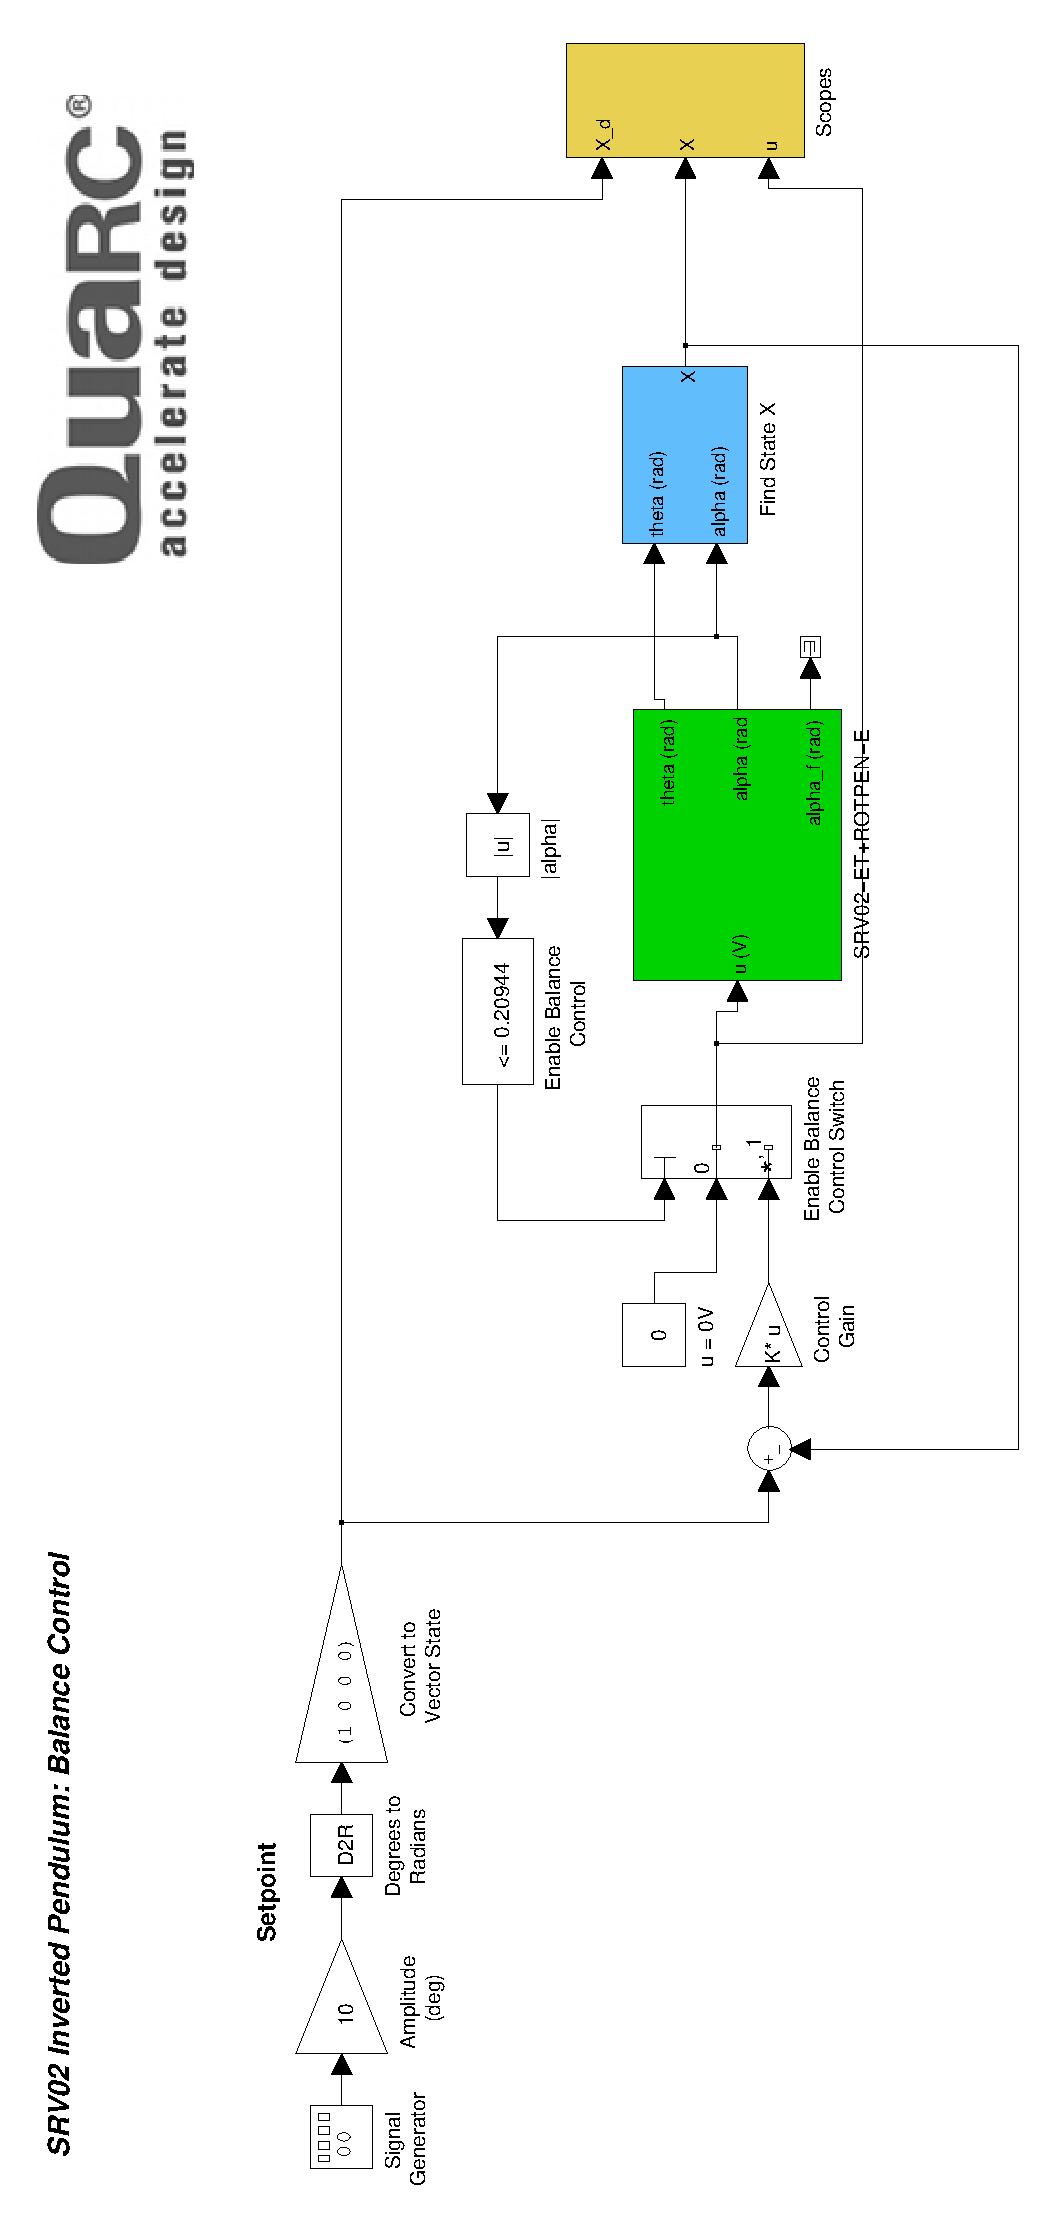
\includegraphics[width=0.5\linewidth,angle=-90]{eps/lab_3/balance_controller.eps}
                        \caption{A Simulink model which interacts with the physical rotary pendulum system and uses state feedback in a small domain about the unstable equilibrium (i.e., inverted pendulum orientation) to balance the inverted pendulum.~\cite{Q-Flex-Beam}}
                        \label{lab3_simulink_balance}
                    \end{figure}
                    \newpage
              \item Record the results of the balancing experiment and plot your data. On one plot, compare the square wave input for the rotor base and the measured rotor base angle, $\theta$. On another plot, include the pendulum angle data, $\alpha$. Does your feedback controller manage to balance the inverted pendulum while tracking the square wave trajectory? What happens if you keep increasing the square wave amplitude, and why does this happen? What happens when you change the poles of the closed-loop system to be more negative in the left half-plane of $\mathbb{C}$ (i.e., designing the feedback gain, $K$, such that the closed-loop poles are much more negative)? For balancing the inverted pendulum, discuss the \emph{trade-offs between designing} the control system such that the poles of the closed-loop system are close to the origin or far in the left half-plane.
                    %\drew{Answer: Yes, it should be able to balance the inverted pendulum while tracking the square wave with amplitude of 10. If the amplitude is increased, then the pendulum angle may exceed the domain of validity of the linearization, and the feedback controller may not be able to balance the inverted pendulum.  Instructors should note that students' answers will vary, as the tension in the slip-gear will change the input required to balance the pendulum. When changing the poles of the closed-loop system by changing $F$, you change the rate of stabilization and the overshoot/undershoot of the stabilization. If one were to place these poles far in the left half-plane, then stabilization would be very immediate, but this immediate response comes at the cost of a large overshoot. In the case of the inverted pendulum, where the linearized system is only valid in a small neighbourhood about the inverted orientation, a large overshoot may be detrimental. Conversely, a very slow stabilization may allow the pendulum to fall outside the linearization's domain of validity, which also causes negative effects. Hence one must design and tune the feedback gain, $K$, for this application such that balancing stabilization is achieved quickly enough without a large overshoot. Here are the plots:
                    %\begin{figure}[htb!]
                    %\centering
                    %	\subfigure{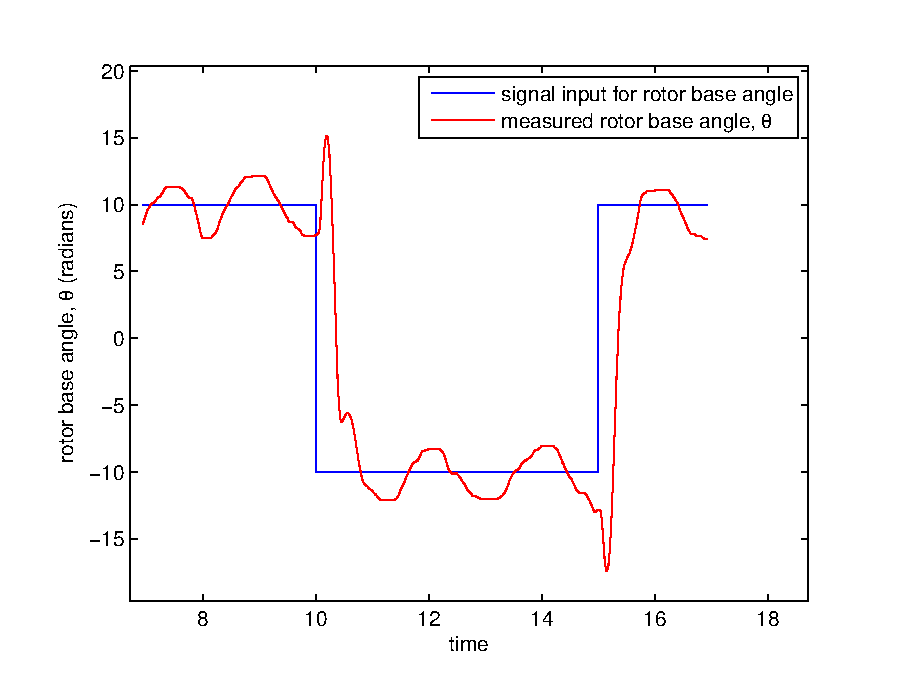
\includegraphics[width=0.4\linewidth]{eps/lab_3/full_feedback_balance_thetas.eps}} \quad
                    %	\subfigure{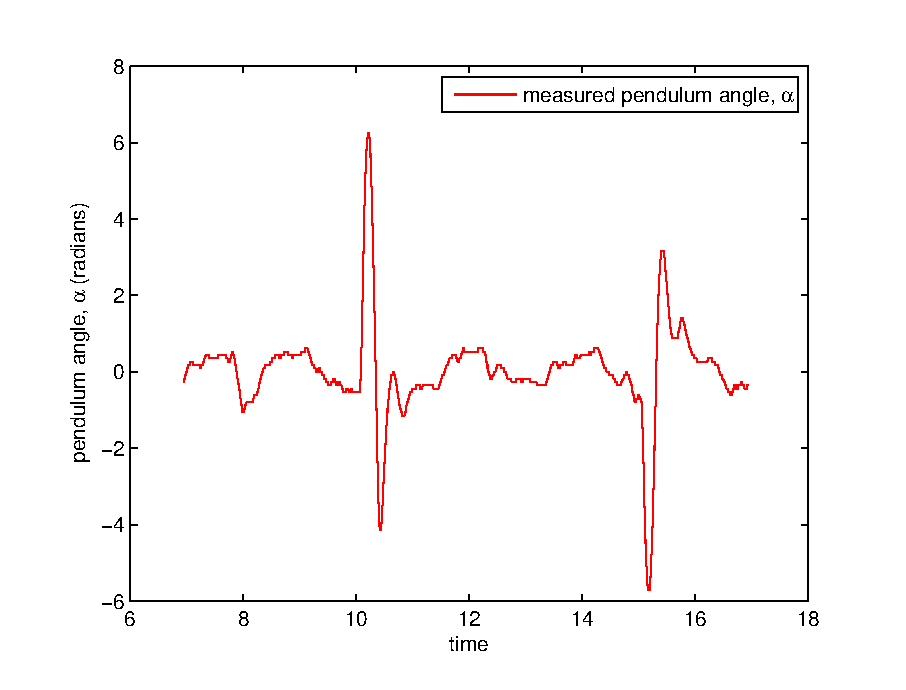
\includegraphics[width=0.4\linewidth]{eps/lab_3/full_feedback_balance_alpha.eps}}
                    %	\caption{(a) A plot of the desired and measured rotor base angle trajectories for the closed-loop feedback controller system while balancing the pendulum in the inverted orientation and while the rotor base tracks a square wave trajectory with amplitude 10, and; (b) a plot of the measured pendulum angle while the physical system tracks this square wave trajectory.}
                    %	\label{fig:lab3_state_feedback_response}
                    %\end{figure}
                    %}
          \end{enumerate}
    \item \textbf{Linear Observer}\label{section:lab3_observer}
          \begin{enumerate}
              \item
                    Recall our linear time-invariant system dynamics
                    \[\mathbf{\dot{x}}(t)=A\mathbf{x}(t)+Bu(t) \quad \quad \quad \mathbf{y}(t)=C\mathbf{x}(t)\]
                    and consider the case where the encoder that reads the pendulum angle is damaged, i.e.,
                    \[C = \left[\begin{array}{c c c c}
                                1 & 0 & 0 & 0 \\
                                0 & 0 & 0 & 0
                            \end{array}\right]\]
                    In this case, you do not have access to one of the system's internal states, $\alpha$. However, you may be able to determine the unknown state by using the system's input and output data. To do this, you will construct a linear dynamical system that produces an estimate of the physical system's state, also known as a \emph{linear state observer}.

                    \textbf{The following questions all concern the \emph{downwards} position.}
              \item When the reader for the pendulum angle is damaged (i.e.\ the matrix \(C\) is as above), can you hope to observe the unknown state $\alpha$ by designing and building an appropriate state observer? What does system detectability mean, and is the system detectable? \textbf{Hint:} Compute the observability matrix of the system.

                    %\drew{Answer: Yes; since the system is observable when 
                    %\[C = \left[\begin{array}{c c c c}
                    %1 & 0 & 0 & 0\\
                    %0 & 0 & 0 & 0
                    %\end{array}\right],\]
                    %it is also detectable, as detectability is a weaker notion of observability. System detectability implies that all of the system's unobservable states are asymptotically stable, but there are no unobservable states for this system.
                    %}
                    One way to \emph{design an observer is by eigenvalue assignment}: the Luenberger observer error, $\tilde{\mathbf{x}}(t)$, governed by the differential equation~\eqref{lab3_equ:luenberger_error}, has a characteristic polynomial chosen by the designer. That is, the observer designer chooses $L$ such that the eigenvalues of $(A-LC)$ are at desired locations $p_1, p_2, \dots, p_n$. This design method has some benefits over other methods, mainly:
                    \begin{itemize}
                        \item theoretically, the observer error can decrease faster if the eigenvalues of $(A-LC)$ are more negative (however, there is a trade-off which you will explore), and;
                        \item if the observed states are being used for state feedback, then the least negative eigenvalue of $(A-LC)$ should be more negative than the eigenvalues of the state feedback system $A-BK$. Loosely speaking, this dictates that the observer dynamics will converge to the unobserved states \emph{faster} than the system dynamics will change these states.
                    \end{itemize}
                    One may notice a similarity between finding a feedback gain $K$ such that $A-BK$ has eigenvalues in $\mathbb{C}^-$ and finding an observer gain $L$ such that $A-LC$ also has eigenvalues in $\mathbb{C}^-$. Recall that the eigenvalues of a matrix and its transpose are the same. The problem of observer design is in fact the \emph{dual} of the state feedback problem, with the following equivalences~\cite{astrom2010feedback}:
                    \begin{align*}
                        (A-LC)^T                      & = A^T - C^T L^T                                  \\
                                                      & \leftrightarrow A - BK                           \\
                        \\
                        A \leftrightarrow A^T \quad B & \leftrightarrow C^T \quad K \leftrightarrow L^T.
                    \end{align*}

                    In Section~\ref{section:lab3_feedback}, you solved for $K$ by using the canonical controllable form and a similarity transformation. In MATLAB, there's a shortcut to solving for $K$ which uses the \emph{place} command. To solve for the feedback gain with desired poles at $\{-2.8 + 2.86i, \; -2.8 - 2.86i, \; -30, \; -40\}$, you can do the following in MATLAB:
                    \[
                        p = [-2.8 + 2.86i \quad -2.8 - 2.86i \quad -30 \quad -40];
                    \]
                    \[
                        K = place(A,B,p);
                    \]

              \item In MATLAB, how could you use the \emph{place} command to design observer gain $L$ such that $A-LC$ has its poles at $p =\{p_1, \; p_2, \; p_3, \; p_4\}$? What is the resulting gain \(L\)? \textbf{Hint:} Use the above duality equations.
                    %\drew{Answer: Using the duality of the observer and feedback design problems, and the equivalences stated above, you could use the MATLAB command
                    %\[
                    %L = place(A',C',p)';
                    %\]
                    %to complete the task.}
          \end{enumerate}

    \item \textbf{Designing \& Validating an Observer}\label{sub section:lab3_observer_design}

          You will now design an observer for the linearized rotary pendulum system, linearized about the \emph{stable equilibrium} (downwards position). You will use the $C$ matrix so that only the rotor base angle, $\theta$, is outputted, as you are studying the case where the encoder reading the pendulum angle is damaged (i.e.\ the \(C\) matrix in the previous section). Figure~\ref{figure:lab3_luenberger_block} shows a Simulink block diagram for a Luenberger observer; you will integrate this observer subsystem into a Simulink model to compare the actual and estimated states.
          \begin{figure}[htb!]
              \centering
              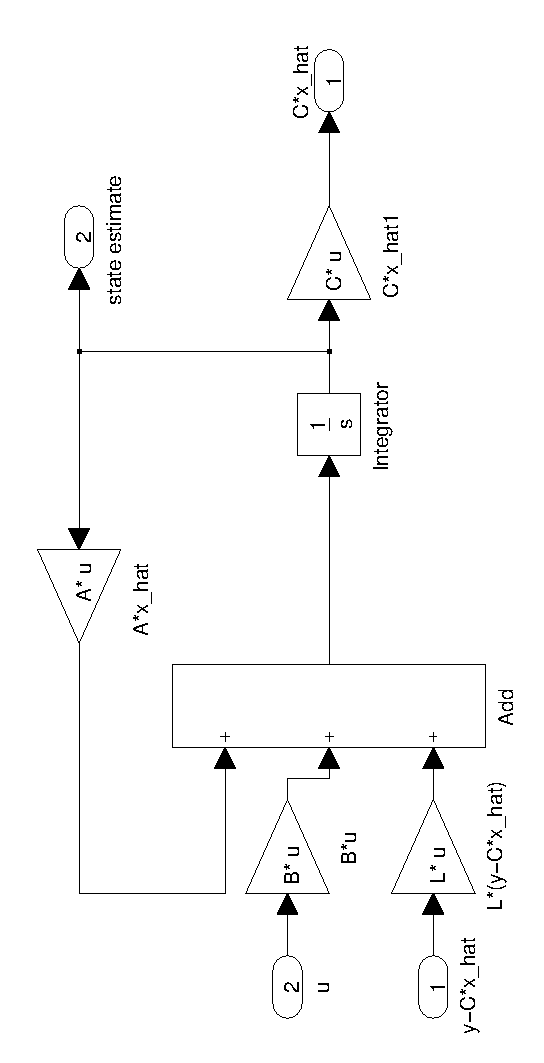
\includegraphics[width=0.4\linewidth,angle=-90]{eps/lab_3/luenberger_subsystem}
              \caption{A Simulink block diagram of a Luenberger observer. This is a subsystem block that can be incorporated into a Simulink model, along with a state-space subsystem block, to compare the estimated and the actual states.}
              \label{figure:lab3_luenberger_block}
          \end{figure}

          Open the Simulink model \textbf{luenberger\_openloop\_model.mdl}. Note that the regular State-Space block is not used to model the linearized rotary pendulum system; in place, we've created a subsystem block that does this, and it is shown in Figure~\ref{figure:lab3_statespace_block} along with the Luenberger observer subsystem block.
          %The state-space subsystem that we've created allows you to access all of the system's states at a given time and output them into the MATLAB workspace, whereas the State-Space block only outputs $y=Cx$. Thus, you must use this subsystem block for the state-space dynamics so that you can compare the actual states and the state estimates produced by your observer.
          \begin{figure}[htb!]
              \centering
              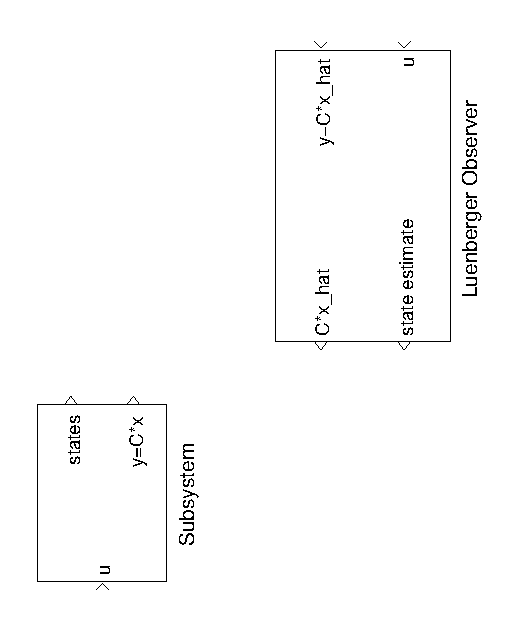
\includegraphics[width=0.4\textwidth,angle=-90]{eps/lab_3/luenberger_openloop_student}
              \caption{A Simulink block diagram of a state-space subsystem \& Luenberger observer subsystem. The state-space subsystem block allows one to output the usual $y=Cx$ output as well as outputting all of the states at each time, making it useful for state estimate validations.}
              \label{figure:lab3_statespace_block}
          \end{figure}

          Connect these two Simulink subsystem blocks so that the observer can estimate the states of the linearized state-space model of the rotary pendulum. Now, add a Signal Generator block, a Sum or Add block, and a DegreesToRadians block to the Simulink model and use a sine signal with amplitude 10 as your input (transforming your input to radians using the DegreesToRadians block). In the state-space subsystem, set the initial conditions (found in the integrator block) of your states to zero (in MATLAB, this is done with the vector $[0;0;0;0]$), and set the initial conditions of your observer subsystem to non-zero values between $[-10,10]$. Make sure to output your states and your state estimates to your workspace using To Workspace blocks.

          \begin{enumerate}
              \item Run various tests using this model while changing the observer's poles in $\mathbb{C}^-$. First, \emph{design and tune your observer} so that the state estimates converges to the actual states very quickly; second, try to achieve state estimates that don't deviate from the actual states too much. \emph{What metrics you would use to evaluate} your observer (and the resulting observer gain design) were it to be used for: state feedback to balance the inverted pendulum, and; monitoring an industrial process where large spikes cause the industrial plant to shut down. \vspace{0.5em}
                    %\drew{Answer: Tuning the observer gain such that the state estimates converge very quickly to the actual states (i.e., the observer poles are far in the left half-plane) comes at the cost of a very large overshoot. Thus, it is important to design the observer gain so that this tradeoff be exploited for a given application. For the inverted pendulum application, since the domain of validity for the linearized system is a small neighbourhood about the inverted orientation, a large overshoot in the pendulum angle state estimation would make the ensuing feedback response overcompensate unnecessarily. Conversely, a slow state estimate convergence can make the ensuing feedback response much to slow to keep the inverted pendulum in the linearized system's domain of validity. This is why this physical stabilization problem is not considered - it is much too finicky to work, and may require techniques other than gain tuning to make it work properly. Some metrics may include overshoot, settling time, energy used in state feedback, etc. For the monitoring application, one would choose to design the observer poles close to the origin since large state estimate overshoots would cost the industrial plant much lost time. The main metric here is overshoot, among other engineering metrics.}

                    Now you will verify that the observer you built for the state-space model works for the physical system. This will help you identify the benefits and drawbacks of different observer tunings for gain $L$. Open the Simulink model \textbf{luenberger\_openloop\_quanser.mdl}. When accessing the rotary pendulum subsystem block, one will notice that the Luenberger observer is nested into this subsystem, as shown in Figure~\ref{figure:lab3_luenberger_openloop_quanser}. This subsystem outputs the measured and the estimated pendulum angle, so that these angles can be compared directly.
                    \begin{figure}[htb!]
                        \centering
                        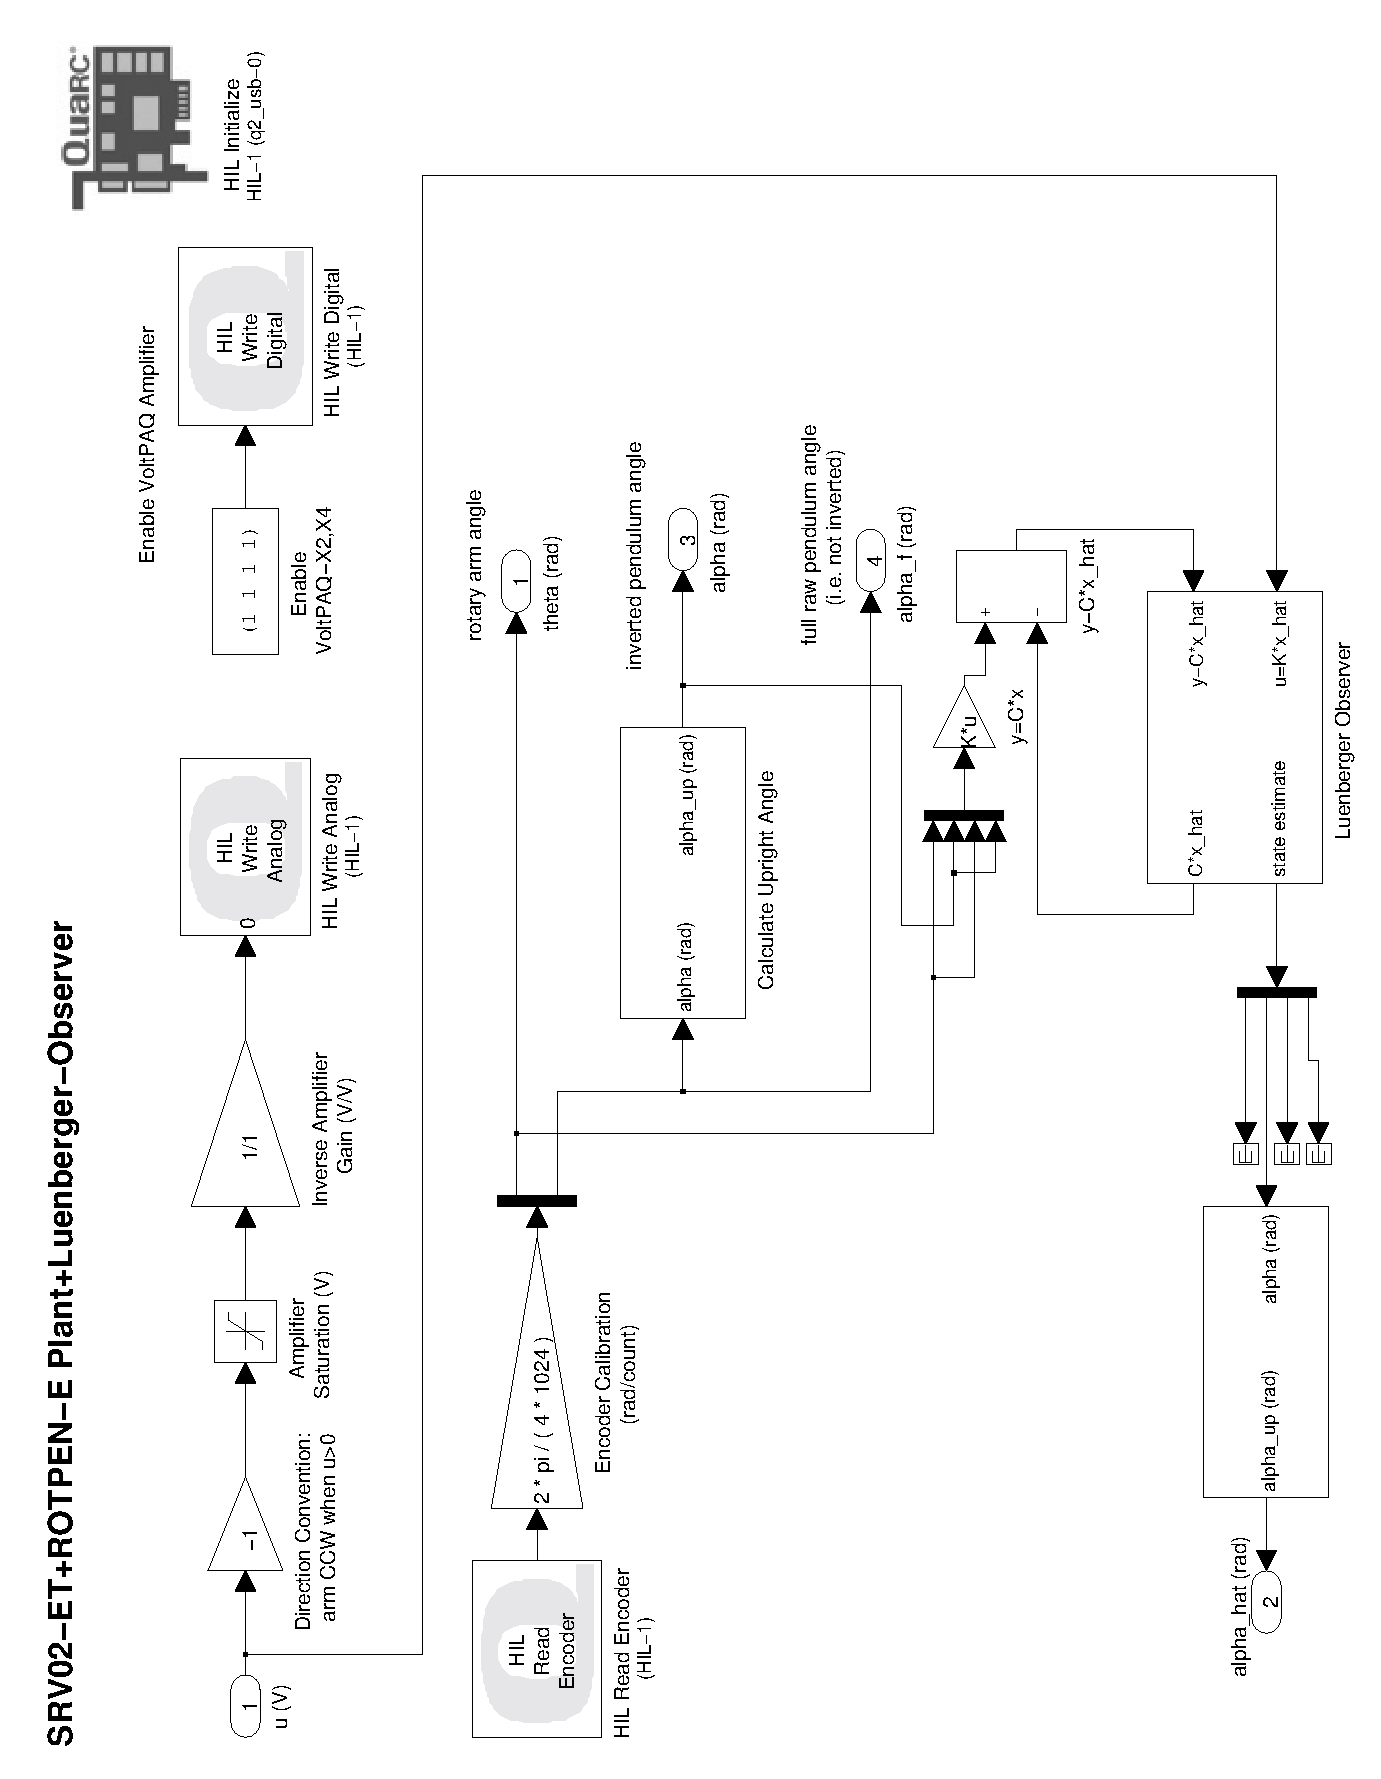
\includegraphics[width=0.6\linewidth,angle=-90]{eps/lab_3/luenberger_openloop_quanser}
                        \caption{A Simulink model of a Luenberger observer estimating \& outputting the pendulum angle, $\hat{\alpha}$, for the physical rotary pendulum system. Note that in the Luenberger observer, measured states $\dot{\theta}$ and $\dot{\alpha}$ are non needed, as they are scaled by $C$.}
                        \label{figure:lab3_luenberger_openloop_quanser}
                    \end{figure}
                    \newpage
              \item Build \& run \textbf{luenberger\_openloop\_quanser.mdl}, with a sine wave input with amplitude of 1 and frequency of 5 $rad/s$. First, use [0,\; 0,\; 0,\; 0] as the initial conditions for the observer. Plot the measured and the estimated pendulum angle, $\alpha$ and $\hat{\alpha}$, with respect to time when your observer has poles $\{-5,\; -6,\; -7,\; -8\}$. Repeat the experiment for observer poles $\{-15,\; -16,\; -17,\; -18\}$, and then for observer poles $\{-45,\; -46,\; -47,\; -48\}$ (creating the same plots for each experiment). Repeat these for the case where the initial conditions of the observer are not identically zero. From these plots, what can you conclude about the relationship between the accuracy of the state estimates produced by your Luenberger observer and \emph{the design and tuning} of the observer gain, $L$? Give two different real-life applications where state observers could be used, and what \emph{metrics} would you develop to evaluate these observers in the setting of their respective applications (specifically look at the relationship between observer behaviour and pole placement via observer gain, $L$).
                    %\drew{Answer: one will note that the observer error after a crest of the sine wave input cannot be completely eliminated for these three observer gains, as some observer error is present in all three plots. The penalty for having very negative observer poles is apparent: while the observer dynamic is very fast, it quickly acts on a control input and then reacts to reduce the estimate output error term ($L(y-C\hat{x}(t)$), and does so frequently. For observer poles at $\{-15,\; -16,\; -17,\; -18\}$, the observer gives a most accurate estimate, but the observer is still a bit too sensitive to control inputs. Due to the constant change in the input signal, the observer estimate error never has time to converge to zero. I will leave the engineering-based responses to be answered by the current TA.
                    %\begin{figure}[htb!]
                    %\centering
                    %\subfigure{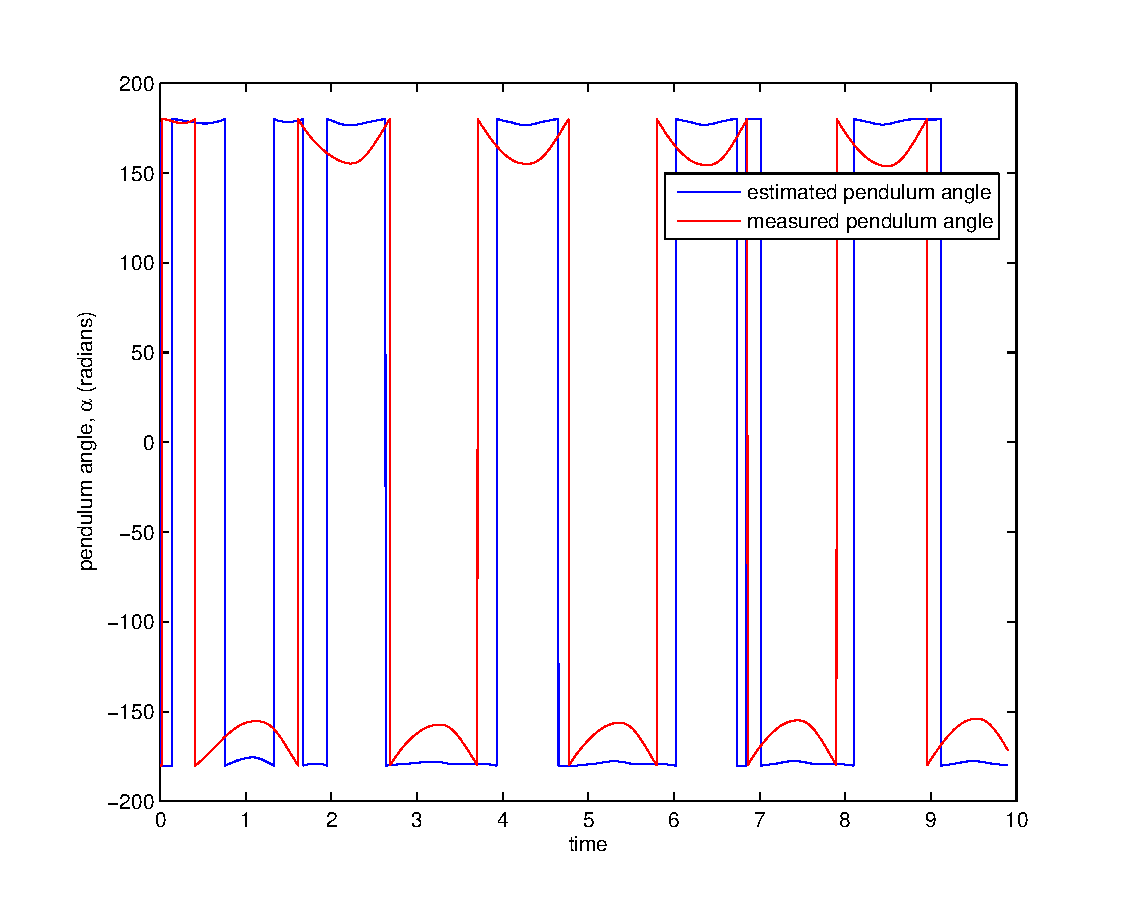
\includegraphics[width=0.4\linewidth]{eps/lab_3/luenberger_openloop_quanser_exp1}}
                    %\subfigure{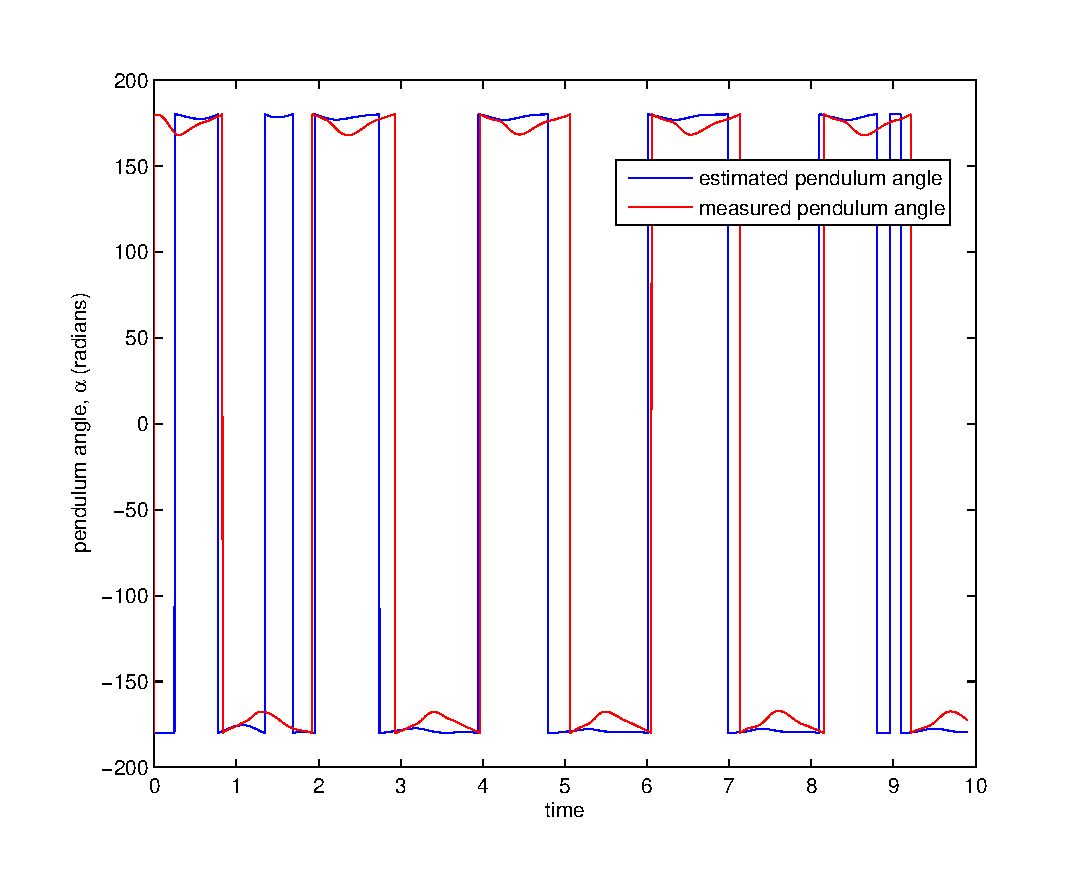
\includegraphics[width=0.4\linewidth]{eps/lab_3/luenberger_openloop_quanser_exp2}}
                    %\subfigure{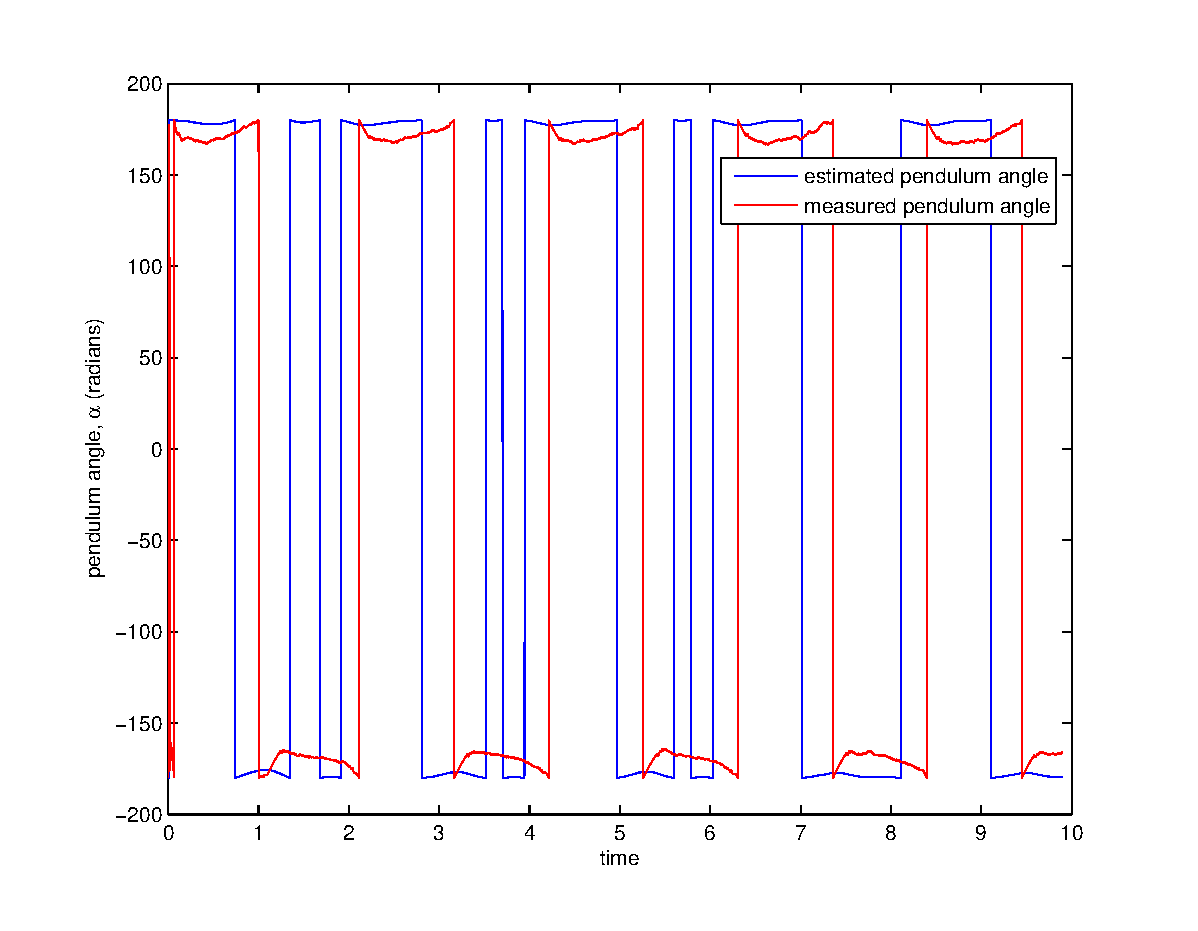
\includegraphics[width=0.4\linewidth]{eps/lab_3/luenberger_openloop_quanser_exp3}}
                    %\caption{Plots comparing the measured and estimated pendulum angle response to a sine wave input of amplitude of 0.5 and frequency of 3 $rad/s$ for observer gains a) $L = \{-5,\; -6,\; -7,\; -8\}$, b) $L = \{-15,\; -16,\; -17,\; -18\}$ and c) $L = \{-45,\; -46,\; -47,\; -48\}$.}
                    %\end{figure}
                    %}
          \end{enumerate}

          %\newpage
          %\subsection{Balance Feedback Control using State Estimate}\label{subsection:lab3_observer_feedback}
          %Now, you'll verify whether you can use your state estimate of $\alpha$, denoted $\hat{\mathbf{\alpha}}$, as well as your measured state, $\theta$, to construct a feedback loop which will make the linearized rotary pendulum system, linearized about the \emph{unstable equilibrium} (i.e., inverted orientation), asymptotically stable.
          %
          %\begin{enumerate}[Questions]
          %\item[Q9:] Is the linearized rotary pendulum system, linearized about $\alpha = 0$ (unstable equilibrium), \emph{detectable}, and why? Is it \emph{stabilizable}, and why? What can be concluded about the viability of using $\hat{\mathbf{\alpha}}$ and $\theta$ as feedback to balance the rotary pendulum in the inverted orientation?\\
          %\drew{Answer: Recall that a system is said to be \emph{detectable} if and only if all of its unstable modes are observable (i.e., if all of its unobservable modes are asymptotically stable). Another way to see this is the following: a system is said to be detectable if $\mathbf{y}(t) \rightarrow 0$ implies that $\mathbf{x}(t) \rightarrow 0$. This is untrue for the state $\alpha$ linearized around the unstable equilibrium, thus a Luenberger observer does not exist for our system.}
          %
          %\drew{A system is said to be \emph{stabilizable} if and only if all of its unstable modes are controllable (i.e., if all of its uncontrollable modes are stable). Note that this definition necessarily implies that if a system is controllable, it is stabilizable (no uncontrollable unstable modes). As you've already shown that this system is controllable, then it follows that it is stabilizable.}
          %
          %\drew{An equivalent definition for stabilizability and detectability is as follows:
          %\begin{itemize}\label{lab3:stabilize_detect_defs}
          %\item given a pair $(A,B)$, we say that $(A,B)$ is \textbf{stabilizable} if there exists $K$ such that $A-BK$ is Hurwitz, and;
          %\item given a pair $(C,A)$, we say that $(C,A)$ is \textbf{detectable} if there exists $L$ such that $A-LC$ is Hurwitz.
          %\end{itemize}}
          %
          %\drew{Recall a result from class that one can use state estimate feedback to place the poles of the closed-loop system at $\mathcal{X}_{(A-LC)} \cdot \mathcal{X}_{(A-BK)}$. Thus, it follows from the alternate definitions of stabilizability and detectability that one can only place the closed-loop poles of the linearized rotary pendulum system in $\mathbb{C}^-$ if it is \textbf{both stabilizable and detectable}, which it is not.}
          %\end{enumerate}

          %Open the Simulink model \textbf{luenberger\_closedloop.mdl}, shown in Figure~\ref{figure:lab3_luenberger_closedloop}. You'll notice that in place of using the measured pendulum angle as was done in Section~\ref{section:lab3_feedback}, the feedback loop uses the estimated pendulum angle. As briefly discussed earlier, when using the state estimate in a feedback loop, one must be careful to choose the eigenvalues of $A-LC$ carefully so that the state estimate dynamics are \emph{faster} than the system's dynamics. A starting point to choose the poles of the observer is to place them five times more negative than the dominating poles of $A-BK$. Recall that the dominating poles are usually those that are closest to the imaginary axis, as they are \emph{slowest} in the sense that they give rise to the longest lasting terms in the transient response of the system.
          %\begin{figure}[htb!]\label{figure:lab3_luenberger_closedloop}
          %\centering
          %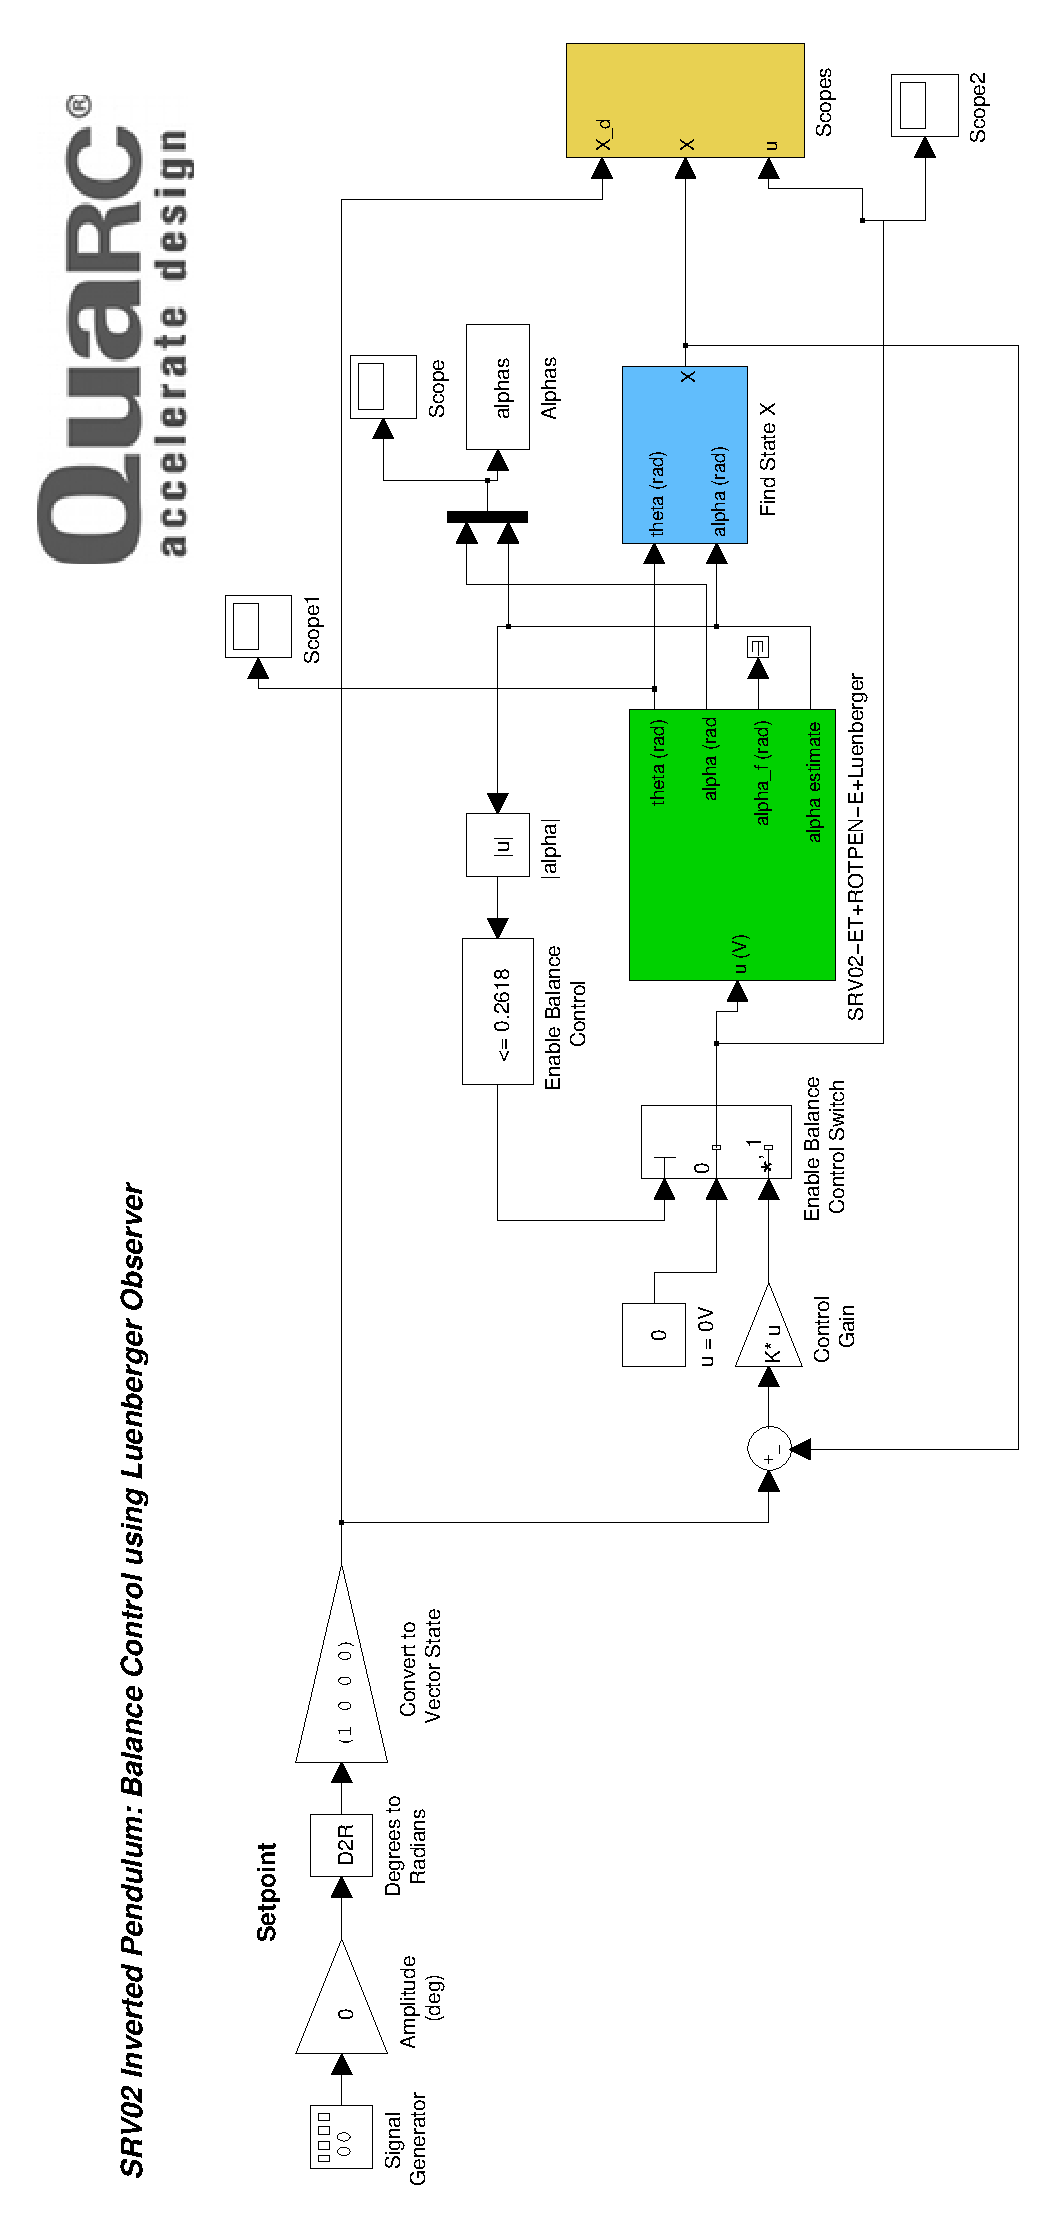
\includegraphics[width=0.5\textwidth,angle=-90]{eps/lab_3/balance_controller_luenberger}
          %\caption{A closed-loop feedback system for the rotary pendulum using partial state feedback and state estimate feedback.}
          %\end{figure}
          %
          %The nature of this experiment is to tune the observer gain, $L$, so that the state estimates are accurate enough to achieve balance control. To tune $L$, you should compare the measured pendulum angle and the estimated pendulum angle using a Scope block (to compare in real-time). After downloading the Simulink model to the target and pressing Run, you can lift the pendulum slightly, observe the error in the pendulum angle estimate via the Scope block, and tune the observer gain appropriately. You should start by setting the poles of $A-LC$ at five times more negative than the dominating pole among $\{-2.8 + 2.86i, \; -2.8 - 2.86i, \; -30, \; -40\}$. \textbf{Note:} you cannot have algebraic multiplicity greater than one when using the \emph{place} command, so you'll have to separate these poles by some numbers that you choose).
          %
          %Once your observer gain is properly tuned, you can lift up the pendulum to the inverted orientation and see if your control system can achieve balancing the pendulum.
          %
          %\begin{enumerate}[Questions]
          %\item[Q8:] First, plot your measured and your estimated pendulum angle with respect to time. Next, plot your control input with respect to time. Did your control system balance the inverted pendulum using partial state feedback and state estimate feedback? Where did you place the poles of your observer gain to achieve this balance control?\\
          %\drew{Answer: Yes, the control system managed to balance the inverted pendulum by using an observer gain of $L = \{-90,\; -92,\; -92.5,\; -93  \}$:
          %\begin{figure}[htb!]
          %\centering
          %\subfigure{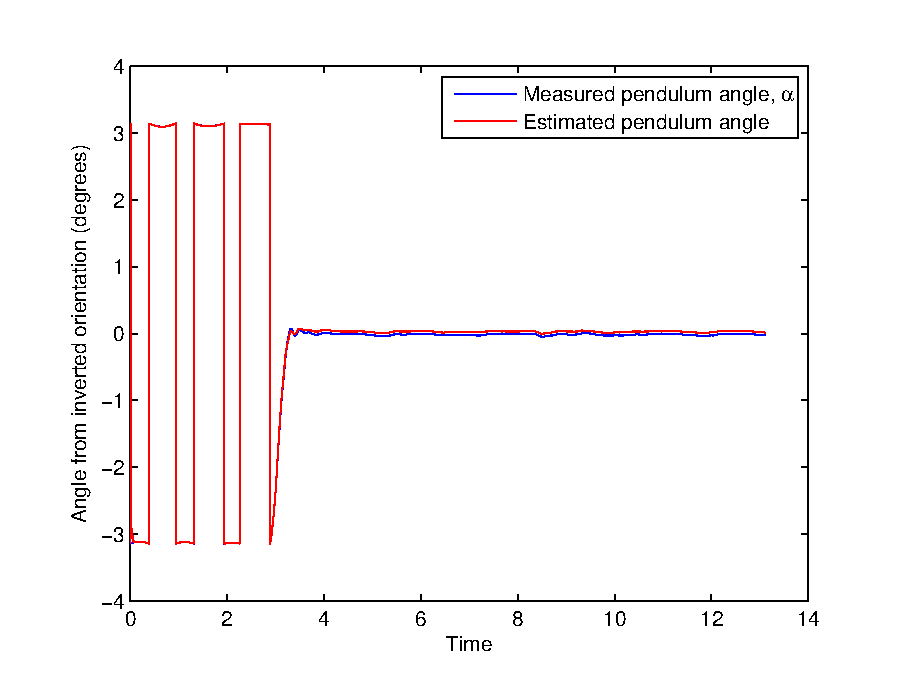
\includegraphics[width=0.5\linewidth]{eps/lab_3/luenberger_closed_loop_alphas}}
          %\subfigure{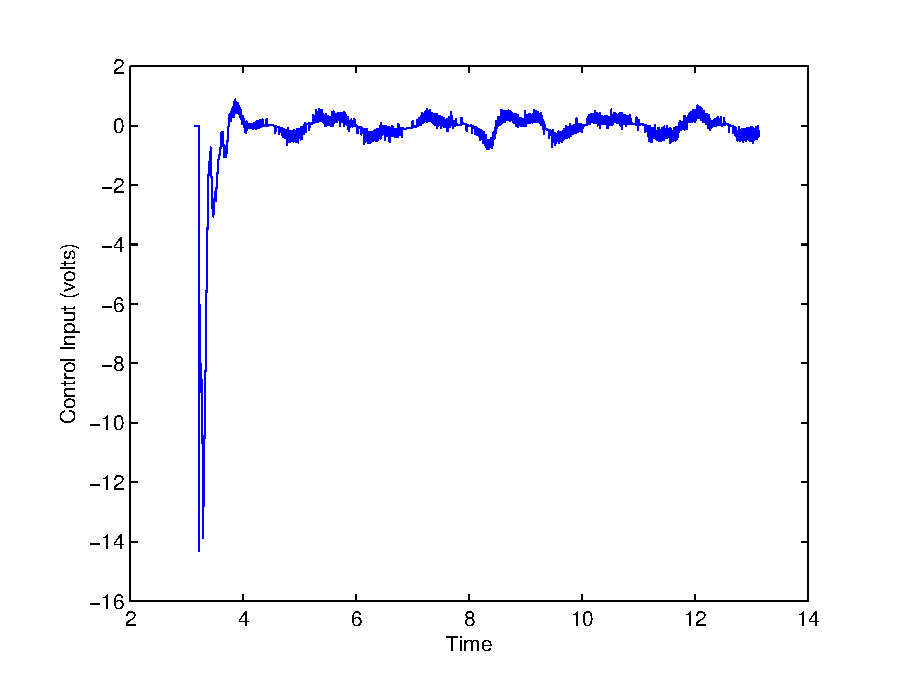
\includegraphics[width=0.5\linewidth]{eps/lab_3/luenberger_closed_loop_input}}
          %\caption{Plots of the estimated and measured pendulum angle, $\alpha$, and the control input. Note that the estimated and measured $\alpha$ agree very well, and one can observe that the control system does balance the inverted pendulum just past three seconds. The control input is constantly adjusting the rotor base to allow the pendulum to stay upright.}
          %\end{figure}}
          %\end{enumerate}
\end{enumerate}

When you have completed the lab, make sure you save your files in a convenient location (e.g.\ on some type of cloud storage).

\section{Deliverables}
Prepare a brief write up describing what you learned from this lab. This does not need to be a formal report, but all material should be presented in a clear and logical manner, with concise descriptions where necessary. Include your answers to all the questions in the lab (these are the lettered sections in the procedure), as well as any requested plots.